\section{Testing the p14\textsuperscript{ARF} explanation of the CDKN2A exception (negative)}
The allele-level section left one explanation untested: low AlphaMissense
scores on CDKN2A might mark alleles that act through p14$^{ARF}$, the second
protein encoded in an alternate reading frame. We tested it directly. From UCSC
hg19 refGene exon coordinates and the hg19 sequence we rebuilt the NM\_000077
(p16$^{INK4a}$) and NM\_058195 (p14$^{ARF}$) coding sequences; both translate
to full-length proteins (156 and 132 aa, Met start, one terminal stop)
and share 206 coding bp in exon 2. Each of the 72 CDKN2A missense SNVs that
match their cBioPortal p16 call (3 excluded as annotated on other
transcripts) was translated in both frames (\texttt{results/cdkn2a\_arf\_alleles.csv}).

\paragraph{The raw association is strong.} Low-AlphaMissense alleles alter
p14$^{ARF}$ in 10/19 cases versus 7/53 for the rest (Fisher OR 7.3,
$p=0.0012$), and inside the shared exon-2 region 10/12 versus 7/33 (OR 18.6,
$p=0.00027$). The most common low-scoring allele, p16 H83Y (48 patients,
AlphaMissense 0.166, ClinVar P/LP), is ARF A97V.

\paragraph{It is explained by reading-frame geometry.} In the shared region
the ARF frame is offset by one base, so a change at p16 codon position 1 alters
ARF in 94\% of alleles and a change at position 2 in 0\%.
Independently, low AlphaMissense scores concentrate at p16 codon position 1
(15/24 alleles vs 4/45 at position 2, $p=4.4\times10^{-6}$). Stratified by codon
position the association vanishes: in the only informative stratum (position
1) ARF is altered in 6/6 high-scoring and 10/11 low-scoring alleles
(Mantel--Haenszel $p=0.76$). \textbf{Verdict:} the data cannot separate an ARF
mechanism from frame geometry; the explanation is not supported, and the
CDKN2A exception is best described as AlphaMissense rating many
codon-position-1 substitutions (e.g.\ H83Y) as benign.

\paragraph{Independent recurrence definition.} We repeated the recurrence test
with residue hotspots from cancerhotspots.org (164 single-residue hotspots in
the four panel genes; statistically defined on large pan-cancer cohorts that
overlap ours, so this is a check of definition, not of data). 355 of 537
panel missense alleles sit at a hotspot residue. AlphaMissense does not
separate hotspot from non-hotspot residues (AUROC 0.519, $p=0.47$), while
REVEL (0.610, $p=2.8\times10^{-5}$) and CADD (0.597, $p=0.00024$) do, reproducing the
AlphaMissense panel ceiling. 13 hotspot alleles (74 of 4,647 hotspot
carriers) score below the likely-pathogenic threshold, led by CDKN2A H83Y.

\begin{figure}[h]\centering
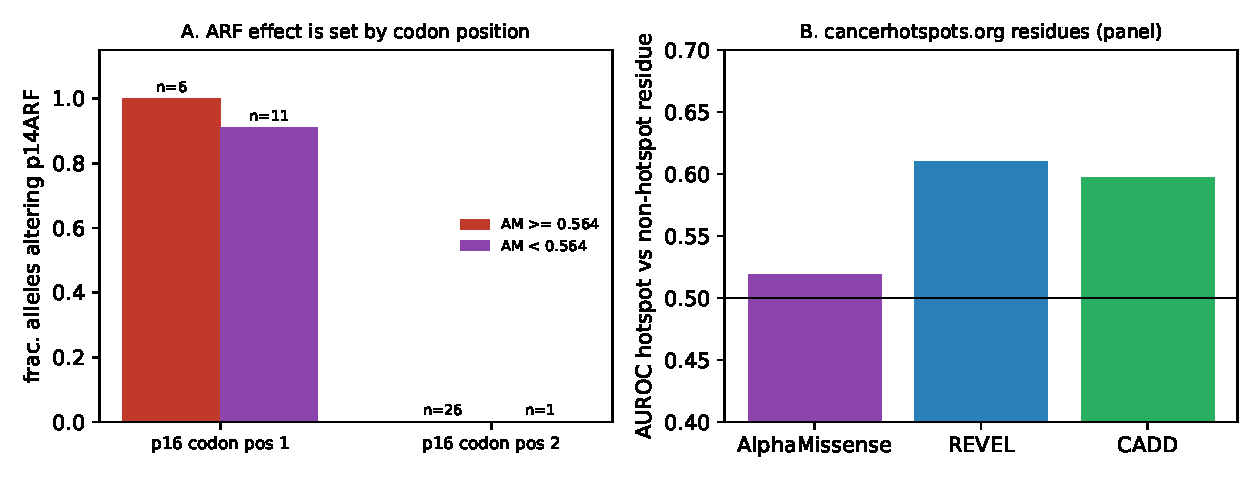
\includegraphics[width=0.85\linewidth]{figs/fig_cdkn2a_arf.pdf}
\caption{A: fraction of CDKN2A missense alleles that alter p14$^{ARF}$, split by
p16 codon position and AlphaMissense class (shared exon-2 region). B:
AlphaMissense does not separate cancerhotspots.org residues from the rest of
the panel; REVEL and CADD do.}\label{fig:cdkn2aarf}\end{figure}
